\section{Caractéristiques d'une force (3 points)}\label{force}

Dans chacun de ces 6 cas donner les caractéristiques de la force représentée. %(direction, sens et point d'application).
La réponse peut être donnée sous la forme d'un tableau ou d'une liste de caractéristiques pour chaque cas.

\begin{center}
%\begin{multicols}{2}
	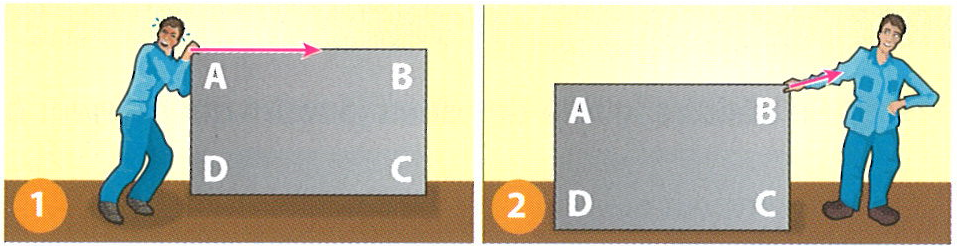
\includegraphics[scale=0.5]{forces_1}
	
	\vspace*{0.5cm}
	
	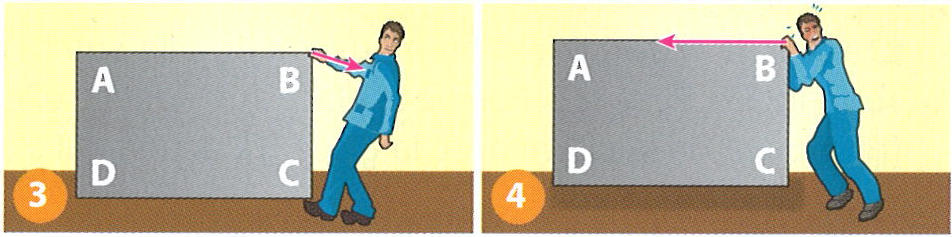
\includegraphics[scale=0.5]{forces_2}
%\end{multicols}

	\vspace*{0.5cm}
	
	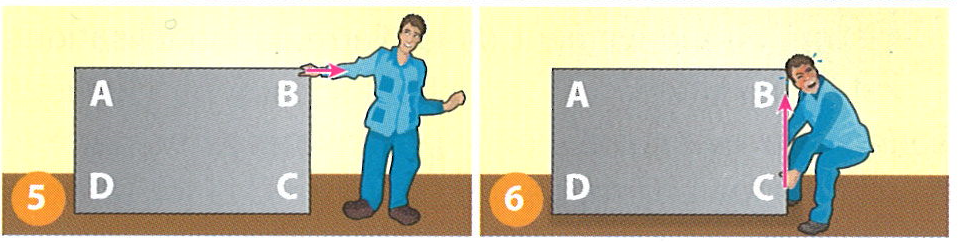
\includegraphics[scale=0.5]{forces3}
\end{center}
